\section{Implementierung}
\label{implementierung}

Der Fokus der Implementierung liegt darauf, eine Ausreichende Infrastruktur zu schaffen, damit die Implementierung einzelner Erweiterungen keine neuen Herausforderungen aufweist, sofern sie zur Installation keine Schritte erfordern, die in der Konzeptionierung nicht berücksichtigt wurden. Die Implementierung einzelner Erweiterungen geschieht also nur exemplarisch um die Funktionalität des Grundgerüsts und des Ansatzes zu demonstrieren.

\subsection{Umsetzung von Erweiterungen im Allgemeinen}
Bei der Definition von und dem Umgang mit Erweiterungen sind einige allgemeine Probleme erschienen, die unabhängig von der konkreten Erweiterung waren. In diesem Unterkapitel wird auf diese Probleme eingegangen und es wird jeweils erläutert, wie sie gelöst werden konnten.

\subsubsection{Probleme mit zyklischen Codeverweisen}
Aus der Konzeptionierung geht hervor, dass es notwendig ist, dass Erweiterungen gegenseitig aufeinander verweisen können, beispielsweise im Rahmen der Definition von Abhängigkeiten oder Exklusivitäten. Außerdem wurde dargestellt, dass Exklusivitäten symmetrisch sind, d.h. dass $A$ zu $B$ genau dann exklusiv ist, wenn auch $B$ zu $A$ exklusiv ist.

Bei der Implementierung von Erweiterungen wurden die Exklusivitäten daher zunächst auch symmetrisch eingetragen. Dies führte jedoch zu dem Problem, dass die Definitionen dieser Erweiterungen zyklisch aufeinander verwiesen haben. Die Definition der Erweiterung $A$ brauchte eine Referenz auf die Erweiterung $B$, aber $B$ konnte nicht ohne eine Referenz auf $A$ erstellt werden.

In JavaScript wird dieses Problem ohne Ausgabe einer Warnung dadurch gelöst, dass eine von beiden Referenzen den Wert \verb|undefined| annimmt, also dass eine von beiden Erweiterungen eine Exklusivität zu \verb|undefined| erhält.

Dasselbe Problem entsteht auch in anderen, gelegentlich notwendigen Situationen. Wenn beispielsweise ein Framework von einer Erweiterung abhängt (weil sie nicht-optional mit installiert wird, wie z.B. Angular nicht ohne TypeScript installiert werden kann) und dann die Deaktivierungsprüfung dieser Erweiterung beinhaltet, dass geprüft werden muss, ob das Framework ausgewählt wurde, erhält man wieder zyklische Verweise innerhalb der Definitionen der Erweiterungen.

Ein Lösungsansatz für dieses Problem wäre, die Definition und die \glqq Füllung\grqq\ der Erweiterungen getrennt voneinander durchzuführen. So könnte erst für jede Erweiterung ein leeres Objekt definiert werden, auf das frei verwiesen werden könnte. Daraufhin würden diese Objekte erst mit den eigentlichen Inhalten der Erweiterung gefüllt.

Dieser Ansatz führt jedoch zu Konflikten mit TypeScript. Da dieselben Variablen verwendet werden sollen, um zunächst leere und dann gefüllte Objekte zu speichern, müssten diese Variablen entweder sehr allgemeine Typdefinitionen haben, die während der weiteren Implementierung zu größeren Aufwänden führen würde, oder sie müssten zu einem Zeitpunkt falsche Typdefinitionen besitzen. Auch dieser Ansatz ist suboptimal, da an entsprechenden Stellen Fehlermeldungen von TypeScript absichtlich deaktiviert oder umgangen werden müssten.

Stattdessen ist für jedes einzelne Problem, das zu einem zyklischen Codeverweis geführt hat, eine eigene Lösung gefunden worden. Die Identifikation von Erweiterungen wurde anhand des Namens der Erweiterung gewährleistet. Dazu muss sichergestellt sein, dass alle Namen einzigartig sind. Da Abhängigkeiten sowieso nicht zyklisch sein dürfen, ergibt sich hier kein Problem. Bei Exklusivitäten wurde auf die symmetrische Spiegelung verzichtet und so konnte durch geschickte Deklaration von Exklusivitäten jeder dadurch bedingte zyklische Codeverweis eliminiert werden.

Dieser Ansatz könnte noch dadurch erweitert werden, dass die Exklusivitäten an separater Stelle (nach der initialen Definition aller Erweiterungen) definiert werden. Da Exklusivitäten ohnehin optional sind (bei der Konzeptionierung wurde festgelegt, dass eine Erweiterung keine Exklusivitäten haben muss), würde dies sich nicht weiter auf die Typdefinition von Erweiterungen auswirken. Außerdem ist auch eine nachträgliche Herstellung der Symmetrie möglich, wenn sie für einen Algorithmus zwingend notwendig ist.

Da durch die nun umgesetzte Lösung das Problem der undefinierten Abhängigkeiten / Exklusivitäten nicht komplett ausgeschlossen werden konnte und zusätzlich noch notwendig geworden ist, dass die Namen von Erweiterungen stets einzigartig sind, wurden Überprüfungen eingeführt, die die Sinnhaftigkeit der definierten Erweiterungen sicherstellen sollen. Konkret wird hier sichergestellt, dass in keiner Liste von Abhängigkeiten oder Exklusivitäten der Wert \verb|undefined| vorkommt und dass alle Erweiterungen einzigartige Namen besitzen.

Diese Sinnhaftigkeitsüberprüfung ließe sich leicht in die normale Ausführung des \gls{CLI}s einbinden, sodass vor jeder Ausführung gewährleistet ist, dass die Erweiterungen sinnvoll definiert sind. Da sich die Erweiterungen aber nach dem Kompilierprozess nicht mehr verändern, würde es auch ausreichen, die Überprüfungen bei der Gelegenheit auszuführen. Dadurch würde bei Nutzenden etwas Rechenleistung gespart werden.

Eine weitere Möglichkeit ist die Ausführung der Überprüfungen im Rahmen der automatisierten Tests. Diese Variante hat den Nachteil, dass es möglich wäre, eine fehlerhafte Version von \gls{GWA} zu veröffentlichen. Da die Ausführung der Tests im Rahmen dieser Arbeit aber bereits nach jeder Änderung automatisch geschieht und sie für zukünftige Fremdbeiträge ebenfalls über GitHub Actions\footnote{\url{https://github.com/features/actions}} automatisiert werden kann, ist dieses Risiko als vernachlässigbar einzustufen.

Da die Einbindung der Überprüfungen in die automatisierten Tests erheblich einfacher ist als die Einbindung in den Kompilierprozess und die Differenz des bleibenden Risikos nicht bedeutend ist, wurde die Einbindung in die automatisierten Tests vorgenommen.

\subsubsection{Prüfung, ob eine Erweiterung ausgewählt worden ist}

\subsubsection{Überprüfung der Umsetzbarkeit der Restriktionen}
Während  der Implementierung verschiedener Erweiterungen ist es versehentlich passiert, dass eine Konstellation von Restriktionen definiert wurde, die einen inneren Widerspruch enthält.

Da zu erwarten ist, dass verschiedene Leute ohne Kenntnis aller anderen Erweiterungen neue Erweiterungen erschaffen oder bestehende Erweiterungen modifizieren werden, sollte verhindert werden, dass versehentlich solche Kombinationen von Restriktionen erzeugt werden. Daher gilt es, mindestens zu jeder Kompilierzeit alle Restriktionen auf ihre Umsetzbarkeit zu überprüfen und im Falle eines Widerspruchs eine Warnung auszugeben. Da im verwendeten Projektumfeld die Ausführung während der Komiplierzeit sich als etwas schwieriger gestaltet hätte und die Überprüfung dieser Restriktionen nicht merklich lange dauert, wurde diese Überprüfung in die Laufzeit des \gls{CLI}s verschoben.

Ein triviales Beispiel einer unmöglichen Kombination von Restriktionen wäre ein Paar von Abhängigkeiten $A$ und $B$, wobei $A$ und $B$ exklusiv zueinander sind und gleichzeitig $A$ von $B$ abhängt. Es können in diesem Beispiel niemals beide Anforderungen gleichzeitig erfüllt werden.

Natürlich lassen sich aber auch kompliziertere Beispiele erzeugen. In Abbildung \ref{fig:impl:dependency_conflict_examples} werden zwei solche Konstellation dargestellt. Bei der einen hängt $A$ von $B$ und $B$ von $C$ ab, aber $A$ ist zu $C$ exklusiv. Diese Kombination von Anforderungen lässt sich ebensowenig wie das erste Beispiel gleichzeitig erfüllen, aber das Problem ist hier nicht sofort offensichtlich. Man muss hierfür erkennen, dass Abhängigkeiten transitiv sind. Ist also die Erweiterung $A$ von $B$ und $B$ von $C$ abhängig, so ist auch indirekt $A$ von $C$ abhängig.

  \begin{figure}
		\centering
		\begin{subfigure}[a]{0.4\linewidth}
			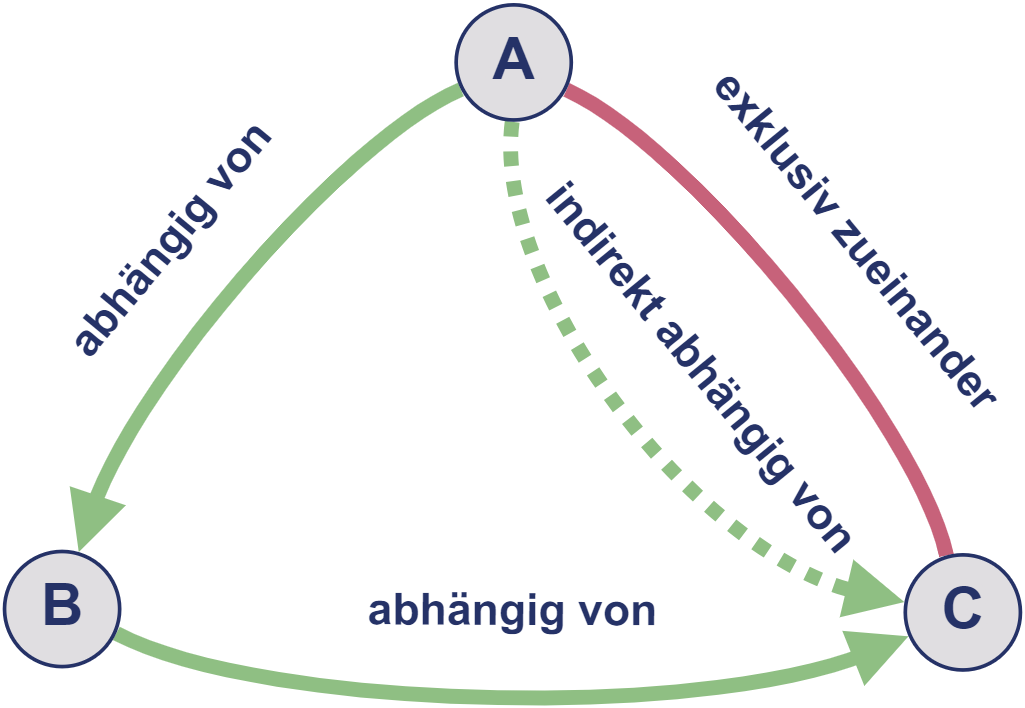
\includegraphics[width=\linewidth]{dependency_example_1.png}
      		\caption{Eine Möglichkeit, wie ein Widerspruch zwischen indirekter Abhängigkeit und Exklusivität entstehen kann.}
		\end{subfigure}
		\begin{subfigure}[a]{0.4\linewidth}
			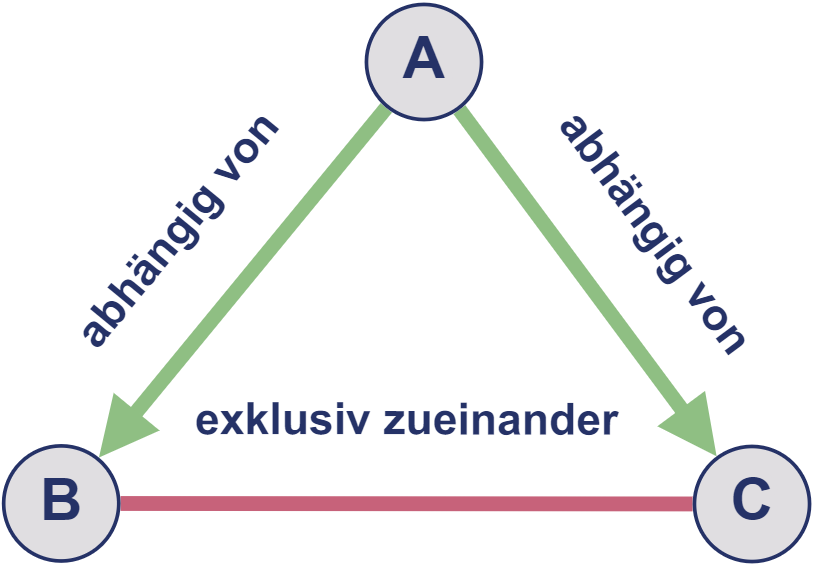
\includegraphics[width=\linewidth]{dependency_example_2.png}
      		\caption{Hier entsteht ein Widerspruch dadurch, dass eine Erweiterung zwei Abhängigkeiten hat, die zueinander exklusiv sind.}
		\end{subfigure}
		\caption{Zwei Graphen zur Veranschaulichung von Konfliktmöglichkeiten zwischen Abhängigkeiten und Exklusivitäten.}
		\label{fig:impl:dependency_conflict_examples}
  \end{figure}

Der zweite in Abbildung \ref{fig:impl:dependency_conflict_examples} dargestellte Konflikt beruht im Gegensatz zu den bisherigen Beispielen nicht darauf, dass eine Erweiterung zugleich (indirekt) abhängig von und exklusiv zu einer anderen Erweiterung ist. Hier wird eine weitere Kategorie von Problemen dargestellt: sind zwei (indirekte) Abhängigkeiten einer Erweiterung zueinander exklusiv, so können nicht beide dieser Abhängigkeiten erfüllt werden. Auch solche Konfigurationen sind also unzulässig.

Aus diesen fachlichen Überlegungen heraus ergibt sich eine erste Lösung. Für jede Erweiterung $E$ sind zunächst alle direkten sowie indirekten Abhängigkeiten zu bestimmen. Für alle diese Abhängigkeiten ist dann zu prüfen, dass zum einen die Abhängigkeit $A$ nicht zu $E$ exklusiv ist, aber auch dass $A$ zu keiner weiteren (indirekten) Abhängigkeit $A'$ von $E$ exklusiv ist.

Bei näherer Betrachtung dieser Lösung lässt sich jedoch einiges an Ineffizienz feststellen. Zum einen werden für jede Erweiterung erneut die transitiven Abhängigkeiten berechnet. Aufgrund eben dieser Transitivität sind jedoch die Berechnungen für alle Erweitungen, die Abhängigkeit einer anderen Erweiterung sind, redundant. Im schlimmsten Fall (nämlich, wenn eine Erweiterung von insgesamt $n$ Erweiterungen von allen anderen Erweiterungen (indirekt) abhängt) ist also genau eine der durchgeführten Berechnungen wirklich notwendig und $n - 1$ Berechnungen werden unnötigerweise durchgefüht. Aus ähnlichem Grund ist auch die Überprüfung der Exklusitivät zweier paarweise unabhängiger (indirekter) Abhängigkeiten häufig überflüssig.

Die Lösung dieser Probleme ergibt sich aus einer theoretischeren Betrachtung des Problems. Wie bereits aus der Verwendung des Begriffs der Transitivität hervorgeht, lassen sich Abhängigkeit und Exklusitivät als mathematische Relationen über der Menge aller Erweiterungen auffassen. Hierbei ist besonders hervorzuheben, dass die Exklusivität symmetrisch ist (ist $A$ zu $B$ exklusiv, so ist auch $B$ zu $A$ exklusiv) während Abhängigkeit nicht symmetrisch ist (im Gegenteil: bei der anfänglichen Analyse von möglichen Bibliotheken, Frameworks etc. ergab sich, dass Abhängigkeit nie symmetrisch zu sein scheint). Allerdings ist Exklusivität a priori nicht transitiv (auch, wenn $A$ zu $B$ und $B$ zu $C$ exklusiv ist, können $A$ und $C$ zusammen verwendet werden), während Abhängigkeit sehr wohl transitiv ist (wie bereits erläutert).

Vor diesem Hintergrund lässt sich erkennen, dass die Bestimmung der (indirekten) Abhängigkeiten der Bestimmung der Transitiven Hülle gleichkommt. Diese kann mittels des Floyd-Warshall-Algorithmus (in der Warshall-Variante) berechnet werden \cite{warshal1_algorithm}. Hierfür muss zunächst ein gerichteter Graph erzeugt werden, in den alle deklarierten Abhängigkeiten als Kante eingefügt werden. Von diesem Graphen wird dann die transitive Hülle bestimmt, in der zwei Knoten $A$ und $B$ genau dann durch eine (von $A$ nach $B$ gerichtete) Kante verbunden sind, wenn die Erweiterung $A$ von $B$ abhängt.

Auch die Relation der Exklusivität lässt sich in einen Graphen überführen. In diesem Graphen gibt es ebenfalls pro Erweiterung einen Knoten und jede Exklusivität wird als Kante dargestellt. Aufgrund der Symmetrie der Exklusivität kann dieser Graph aber ungerichtet sein.

Das Problem der Überprüfung der Restriktionen reduziert sich nun darauf, sicherzustellen, dass es zwischen zwei Knoten (also zwischen zwei Erweiterungen) in maximal einem der beiden Graphen eine Kante gibt, wobei die Richtung keine Rolle spielt (denn wenn die Knoten exklusiv zueinander sind, darf es zwischen beiden keine Abhängigkeit geben -- egal, in welche Richtung).

Anders formuliert, darf es im Graphen der Exklusivitäten keine Kante $\{A, B\}$ geben, für die in der transitiven Hülle der Abhängigkeiten die Kante $(A, B)$ oder die Kante $(B, A)$ existiert. Aufgrund dessen, dass die transitive Hülle gerichtet ist, gibt es darin doppelt so viele Kanten wie in dem Graphen der Exklusivitäten. Außerdem liegt sie als Adjazenzmatrix vor, während die Exklusivitäten als Kantenliste vorliegen. Somit kann bei $m$ Exklusivitäten in $\mathcal{O}(m)$ über die Exklusivitäten iterieren und jeweils in $\mathcal{O}(1)$ die Existenz einer (transitiven) Abhängigkeit prüfen. Die Umkehrung, also die Iteration über Abhängigkeiten und dann die Prüfung der Existenz einer Exklusivität, würde bei $n$ Erweiterungen einen Aufwand von $\mathcal{O}(n^2)$ verursachen. Wenn man vorher die Kantenliste der Exklusivitäten in $\mathcal{O}(n^2)$ in eine Adjazenzmatrix überführt, ist die anschließende Existenzprüfung auch wieder in $\mathcal{O}(1)$ möglich, aber insgesamt

Der Algorithmus von Floyd-Warshall sorgt dafür, dass diese Überprüfung eine asymptotische Laufzeit von $\mathcal{O}(n^3)$ hat. Da die oben beschriebenen Probleme in beliebiger Tiefe von Abhängigkeiten auftreten können, ist jedoch die Bestimmung der transitiven Hülle nicht vermeidbar. Allerdings ist damit zu rechnen, dass die Anzahl aller Erweiterungen stets kleiner als $100$ sein wird (andernfalls würde die Benutzbarkeit des Programms möglicherweise stark eingeschränkt). Daher ist diese Laufzeit in diesem Fall als unbedenklich einzustufen.

Da auch diese Überprüfung sich lediglich auf die Definitionen der Erweiterungen verlässt, wird auch sie in die Ausführung der automatisierten Tests eingebunden, damit sichergestellt werden kann, dass keine fehlerhaften Erweiterungsdefinitionen veröffentlicht werden.

\subsubsection{Überprüfung der getroffenen Auswahl von Erweiterungen}
Um die getroffene Auswahl an Erweiterungen auf die Einhaltung aller Restriktionen hin zu überprüfen, wurde ebenfalls zunächst eine fachliche Lösung gefunden. Für jede der ausgewählten Erweiterungen sind alle Abhängigkeiten und Exklusivitäten durchzugehen. Ist eine Abhängigkeit nicht mit ausgewählt worden oder ist eine Exklusivität mit ausgewählt worden, so ist (genau dann) die Kombination ungültig.

Die Laufzeit dieses Vorgehens liegt für $n$ mögliche Erweiterungen in $\mathcal{O}(n^3)$ (mit Möglichkeit der Reduktion auf $\mathcal{O}(n^2)$). Dies liegt daran, dass zunächst über jede der (maximal $n$) ausgewählten Erweiterungen und dann über jede der Abhängigkeiten und Exklusivitäten iteriert werden muss. Da eine Erweiterung niemals zu einer Abhängigkeit exklusiv sein kann, beträgt die Summe der Abhängigkeiten und Exklusivitäten maximal $n$. Somit ist bereits eine Laufzeit von $\mathcal{O}(n^2)$ erreicht worden.

Nun bleibt noch die Prüfung, ob eine Abhängigkeit bzw. Exklusivität ausgewählt worden ist oder nicht, d.h. ob sie in der Liste der ausgewählten Erweiterungen liegt oder nicht. Im Falle einer normalen Liste läge die Laufzeit dieser Überprüfung bei $\mathcal{O}(n)$, da die im schlimmsten Fall die gesamte Liste überprüft werden müsste. Allerdings kann man diese Information auch als Liste bool'scher Werte speichern, wobei unter jedem Index genau eingetragen ist, ob die Erweiterung mit demselben Index in der Liste aller möglichen Erweiterungen ausgewählt worden ist. So wäre die Überprüfung der Auswahl einer einzelnen Erweiterung in $\mathcal{O}(1)$ möglich und würde die Gesamtlaufzeit nicht weiter beeinflussen.

Ähnlich wie bei der Überprüfung der Umsetzbarkeit aller Restriktionen lässt sich jedoch auch für dieses Problem eine graphentheoretische Lösung finden. Da bereits Graphen bestimmt wurden, in denen Kanten für Abhängigkeit und Exklusivität eingetragen sind, können diese zunächst kopiert und dann zur Überprüfung dieses Problems verwendet werden. Die Kopie erfolgt in $\mathcal{O}(n^2)$, da eine $n \times n$-Adjazenzatrix und eine Kantenliste mit maximal Länge $n^2$ kopiert werden müssen.

Im Graphen der Abhängigkeiten sind Kanten nun als noch unerfüllte Bedingungen anzusehen. Die Streichung einer Kante bedeutet somit, dass die entsprechende Bedingung erfüllt ist. Nun ist über jede mögliche Erweiterung zu iterieren. Falls sie ausgewählt worden ist, so sind auf sie eingehende Kanten aus dem Graphen der Abhängigkeiten zu streichen. Andernfalls (d.h. wenn sie nicht ausgewählt worden ist) ist ihr Knoten mitsamt seiner ausgehenden Kanten zu streichen. Es sind genau dann alle Abhängigkeiten erfüllt, wenn nach der Iteration über alle möglichen Erweiterungen keine Kanten mehr in dem Graphen vorhanden sind.

Ähnlich ist für die Exklusivitäten zu verfahren. In diesem Graphen bedeutet die Existenz einer Kante, dass die zugehörige Exklusivität in der aktuellen Auswahl noch nicht ausgeschlossen werden konnte. Während über alle Erweiterungen iteriert wird, kann also für jede nicht ausgewählte Erweiterung der zugehörige Knoten zusammen mit seinen (ungerichteten) Kanten gestrichen werden. Auch die Exklusivitäten sind alle genau dann erfüllt, wenn sich am Ende der Iterationen keine Kante mehr im Graphen befindet.

Der erste Aspekt der Laufzeit dieser Verfahren ergibt sich dadurch, dass die Graphen in verwendbarer und modifizierbarer Form vorliegen müssen (d.h. als neu angelegte Adjazenzmatrizen). Die im letzten Kapitel berechnete Adjazenzmatrix der Abhängigkeit muss also lediglich kopiert werden, während der Graph der Exklusivität in eine Adjazenzmatrix überführt werden muss. Dies kann in $\mathcal{O}(n^2)$ geschehen.

Danach muss über jede Erweiterung iteriert werden und ggf. (also falls sie nicht ausgewählt wurde) die zugehörige Zeile und Spalte der Adjazenzmatrix modifiziert werden. Anschließend muss die gesamte Matrix auf die Existenz von Kanten hin überprüft werden. Beide Schritte geschehen nacheinander in jeweils $\mathcal{O}(n^2)$. Somit fordert der gesamte Prozess eine Laufzeit von $\mathcal{O}(n^2)$.

Alternativ zu den Adjazenzmatrizen könnten auch Kantenlisten verwendet werden. Dann müsste aber für die Löschung von Knoten, die in beiden Prozessen maximal für jede Erweiterung vorkommen könnte, jeweils die gesamte Liste durchlaufen werden. Es entstünde also auch hier ein Aufwand von $\mathcal{O}(n^2)$.

Die Betrachtung der Graphentheoretischen Lösung ergibt also in diesem Fall keine Verbesserung der Laufzeit. Nach persönlichem Empfinden ist die erste Lösung jedoch leichter zu verstehen und wurde angesichts der gleichen Laufzeit aufgrund dieses Kriteriums ausgewählt und umgesetzt.

\subsection{Umsetzung des Dialogs}
\subsubsection{Stellen allgemeiner Fragen}
\subsubsection{Übergabe des Dialogs an Erweiterungen}

\subsection{Installation von Erweiterungen}
\subsubsection{Erzeugung von TypeScript- und JavaScript-Dateien}
\subsubsection{Framework-spezifische Codegeneration}
\subsection{Betriebssystemspezifische Probleme}
\subsection{Testgetriebene Entwicklung}